\documentclass[10pt,a4paper]{article}
\usepackage{preamble}
\usepackage{listings}

\definecolor{codegreen}{rgb}{0,0.6,0}
\definecolor{codegray}{rgb}{0.5,0.5,0.5}
\definecolor{codepurple}{rgb}{0.58,0,0.82}
\definecolor{backcolour}{rgb}{0.95,0.95,0.95}
\renewcommand{\lstlistingname}{Code}% Listing -> Code
\renewcommand{\lstlistlistingname}{List of \lstlistingname s}% List of Listings -> List of Codes
\lstdefinestyle{mystyle}{
    backgroundcolor=\color{backcolour},
    commentstyle=\color{codegreen},
    keywordstyle=\color{magenta},
    numberstyle=\tiny\color{codegray},
    stringstyle=\color{codepurple},
    basicstyle=\ttfamily\footnotesize,
    breakatwhitespace=false,
    breaklines=true,
    captionpos=b,
    keepspaces=true,
    numbers=left,
    numbersep=3pt,
    showspaces=false,
    showstringspaces=false,
    showtabs=false,
    tabsize=3
}
\lstset{style=mystyle}

\def\FS{Formelsammlung}
\def\Fach{Regelungstechnik}
\def\FachAkz{RT}
\title{\FS \ \Fach}
\author{Bastian Nagler}
\date{\today}
\def\Semester{SoSe 26}

\begin{document}

\pagenumbering{gobble}
\begin{titlepage}
\thispagestyle{empty}

	\begin{center}
		\vspace*{\stretch{0.5}}
		
\includegraphics[width=0.5\textwidth]{./Figures/Logo/OTHR_FakEI_Logo.png}\\
		\vspace*{\stretch{0.25}}
		\Huge
		\textsc{\FS}\\
		\textsc{\Fach \hspace*{1pt} (\FachAkz)}\\
		\large
		\vspace*{\stretch{0.5}}
		{nach Vorlesungsunterlagen von\\ Prof. Dr.-Ing. C. Brüdigam}\\
		\vspace*{\stretch{0.5}}

\vspace*{\stretch{2}}
{\renewcommand{\arraystretch}{1.5}
\begin{tabular}{l l}
	\href{https://github.com/maxibaxi16/RT_Formelsammlung}{Originalversion:} & \hspace{4cm} Maximilian Binninger\\
	\href{https://github.com/BastianNagler/RT_Formelsammlung}{Überarbeitet:} & \hspace{4cm} Bastian Nagler\\
    %Matrikelnummer:  & \hspace{4cm}\MatNr\\
    Letzter Stand:  & \hspace{4cm} \textsc{\Semester}  \\
    Lizenz:  & \hspace{4cm} GPLv3
\end{tabular}
}
\vspace*{\stretch{1}}

\end{center}
\end{titlepage}


\newpage

\tableofcontents\clearpage

\pagestyle{fancy}
%\renewcommand{\sectionmark}[1]{\markboth{#1}}
\fancyhead[L]{Bastian Nagler}
\fancyhead[R]{\nouppercase{\leftmark}}
%\rhead{\leftmark}
%\cfoot{\vspace{-20pt}\thepage}
\pagenumbering{arabic}
\fancyfoot[c]{\thepage \hspace{1pt} von \pageref{LastPage}}
% \setlength{\columnsep}{1pt}
\raggedcolumns
\begin{multicols*}{2}

	\section{Grundlagen}

\subsection{Gleichungen zur Modellbildung}
	Kräftegleichungen:
	\begin{mdframed}[style=exercise]
		Federkraft: \(F_F\) = \(k_F \cdot x\)\\
		Dampfkraft: \(F_D\) = \(k_D \cdot v\) = \(k_D \cdot \dot{x}\)\\
		Trägheitskraft: \(F_{Tr}\) = \(m\cdot a\) = \(m\cdot \ddot{x}\)\\
		Erdanziehungskraft: \(F_G\) = \(m\cdot g\)
	\end{mdframed}
	Moment Gleichungen:
	\begin{mdframed}[style=exercise]
		Widerstandsmoment: \(M_w = k_D \cdot \omega\)\\
		Trägheitsmoment: \(M_{TR} = J \cdot \dot{\omega}\)
	\end{mdframed}
	Spannungsgleichung:
	\begin{mdframed}[style=exercise]
		\[
			U = L\cdot \frac{di}{dt}+i\cdot R+\frac{1}{C} \cdot \int i
		\]
	\end{mdframed}

	Rotation in Flüssigkeit:
	\[
		M=M_{\texttt{Träg}}+M_{\texttt{Brems}}=J \cdot \dot{\omega} +k_{\texttt{Flüssigkeit}} \cdot \omega
	\]

\subsection{Mathematische Grundlagen}
	Für kleine Winkel \(\alpha\) gilt: sin(\(\alpha\)) = \(\alpha\)\\
	\\
	Partialbruchzerlegung (siehe Papula s.157ff)\\
	\\
	Anfangswertsatz: \(x(t \rightarrow +0)=\lim _{s \rightarrow \infty} s \cdot X(s)\)\\
	Endwertsatz: \(x(t \rightarrow \infty)=\lim _{s \rightarrow 0} s \cdot X(s)\)

\subsection{Linearisierung um Arbeitspunkt}
	\begin{align*}
		x_{a}(t) &= x_{a,AP} + \Delta x_{a}(t) \\ 
		&\approx f(x_{e1,AP}, ..., x_{en,AP}) + \sum_{m=1}^{n} \left. \frac{\partial f}{\partial x_{em}} \right|_{AP} \cdot \Delta x_{em}(t)
	\end{align*}

\subsection{Eigenschaften von LTI-Systemen}
	\begin{mdframed}[style=exercise]
		\begin{enumerate}
			\item BIBO-Stabilität {\footnotesize (Bounded Input / Bounded Output)}\\
				\(\abs{y(t)} < \infty \qquad \text{für} \quad \abs{x(t)} < \infty\)
			\item Linearität\\
				\(f\qty{\sum_{k=1}^{N}a_n x_n(t)}=\sum_{n=1}^{N}f\qty{a_n x_n(t)}\)
			\item Zeitinvarianz\\
				\(f\qty{x(t-t_0)} =y(t-t_0)\)
			\item Kausalität\\
				\(x(t)=0 \; , \; y(t)=0 \qquad \text{für} \quad t < 0\)
		\end{enumerate}
	\end{mdframed}

\subsection{Systemantwort}
	\begin{mdframed}[style=exercise]
		\textbf{Sprungantwort} \((x = \sigma)\)
		\begin{align*}
			g(t) &= \mathcal{L}^{-1}\qty{G(s)} = \mathcal{L}^{-1}\qty{\frac{F(s)}{s}}\\
			g(t) &= \int_{0}^{t} h(\tau) \dd{\tau}
		\end{align*}
	\end{mdframed}
	\begin{mdframed}[style=exercise]
		\textbf{Impulsantwort} \((x = \delta)\)
		\begin{align*}
			h(t) &= \int_{-\infty}^{\infty} x(\tau) \delta(t-\tau) \dd{\tau}\\
			h(t) &= \mathcal{L}^{-1}\qty{F(s)}\\
			h(t) &= \frac{d}{\dd{t}} g(t)
		\end{align*}
	\end{mdframed}

\subsection{Abtasttheorem}
	Durch die Abtastung wird das Spektrum von \(f(t)\) unendlich oft um die Frequenzen \(n\cdot \omega_a\) reproduziert.
	\begin{mdframed}[style=exercise]
		\begin{align}
			F_A(\omega) &= \frac{1}{T_A} \sum_{n=-\infty}^{\infty} F(\omega-n\omega_A)\\
			2\omega_g &\leq \omega_A
		\end{align}
	\end{mdframed}
	\section{Systemtechnik}
\subsection{Modellbildung}
	Hinweise zum aufstellen der Differentialgleichung eines Systems:
	\begin{mdframed}[style=exercise]
		\begin{enumerate}
			\item Bestimmung der Ein- und Ausgangsgrößen
			\item Suche nach dem beschreibenden Gleichgewicht
			\item In der Gleichung dürfen nur Konstanten, sowie die Ein- und
				Ausgangsgrößen in beliebiger Ableitung vorkommen
			\item Andere Variablen müssen durch erlaubte Größen ersetzt werden\\
				\footnotesize
				(Dazu können i.a. physikalische Gleichungen benutzt werden)
		\end{enumerate}
	\end{mdframed}

\subsection{Signalflussplan/Blockschaltbild}
	Erzeugung des Signalflussplans aus der Zugehörigen DGL.
	\begin{mdframed}[style=exercise]
		\begin{enumerate}
			\item für technische Realisierung gilt: \(m \le n\);

			\item DGL. nach höchster Ableitung der Ausgangsgröße auflösen

			\item höchste Ableitung der Ausgangsgröße geht auf den Eingang des ersten Integrators\\
				\footnotesize
				(Laplace-Trans ersetzt Integrieren mit \(\frac{1}{s}\))
		\end{enumerate}
	\end{mdframed}
	\begin{center}
		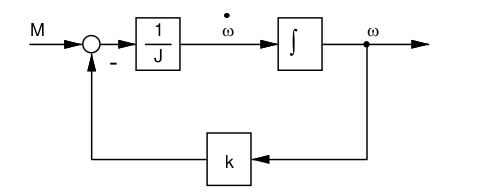
\includegraphics[width=0.96\columnwidth]{Figures/systemtechnik/Signalflussplan12.png}
	\end{center}

	\begin{mdframed}[style=exercise]
		Erzeugung des Signalflussplans eines Systems mit der DGL.:
		\begin{align*}
			& a_{n} \overset{(n)}{x}_{a}+\ldots+a_{2} \ddot{x}_{a}+a_{1} \dot{x}_{a}+a_{0} x_{a} \\
			= & b_{m} \overset{(m)}{x}_{e}+\ldots+b_{2} \ddot{x}_{e}+b_{1} \dot{x}_{e}+b_{0} x_{e}
		\end{align*}
		\centering
		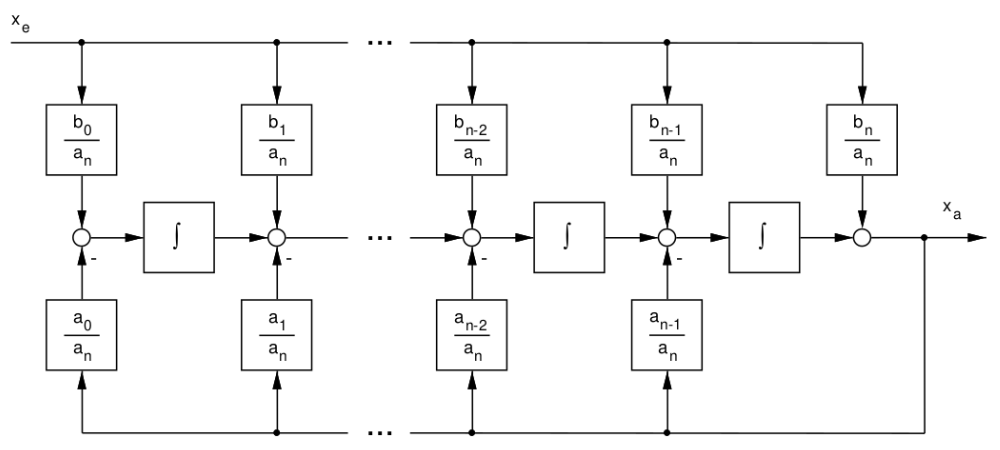
\includegraphics[width=\columnwidth]{Figures/systemtechnik/SFmitDGL.png}
		Falls \(m < n \), sind alle höheren \(b_\mu = 0\) zu wählen.
	\end{mdframed}

\subsection{Übertragungsfunktion F(s)}
	\begin{align*}
		F(s) = \frac{X_a(s)}{X_e(s)}
	\end{align*}

\subsubsection{F(s) aus DGL}
	
\begin{mdframed}[style=exercise]
	\begin{align*}
		& a_{n} \overset{(n)}{x}_{a}+\ldots+a_{1} \dot{x}_{a}+a_{0} x_{a} = b_{m} \overset{(m)}{x}_{e}+\ldots+b_{1} \dot{x}_{e}+b_{0} x_{e}\\
		& \Rightarrow F(s) = \frac{b_{m} s^{m}+\ldots+b_{2} s^{2}+b_{1} s+b_{0}}{a_{n} s^{n}+\ldots+a_{2} s^{2}+a_{1} s+a_{0}}
	\end{align*}
\end{mdframed}

\subsubsection{F(s) in Pol- und Nullstellenform}

\[
	F(s)=Q \cdot \frac{\prod_{\mu=1}^{m}\left(s-s_{N \mu}\right)}{\prod_{v=1}^{n}\left(s-s_{P V}\right)}
	\qquad \texttt{mit } Q = \frac{b_m}{a_n}
\]

\begin{mdframed}[style=exercise]
	Pole in der rechten Halbebene führen zu einem instabilen System. Diese können nicht durch Nullstellen kompensiert werden.

	Pole bewirken ein zeitverzögertes Verhalten. Je weiter links sie sich befinden,
	desto schneller ist der Einschwingvorgang.\\
	$\Rightarrow$ Wenn Pole deutlich weiter links liegen als andere andere, kann man sie ohne
	großen Fehler vernachlässigen.
\end{mdframed}
\begin{mdframed}[style=exercise]
	Nullstellen bewirken ein differenzierendes Verhalten (Beschleunigung des Systems)
	Einfluss weit links in der s-Ebene kann häufig vernachlässigt werden.
\end{mdframed}

\newcolumn
\subsection{Signalflussplan Algebra}
\begin{itemize}[leftmargin=*]
	\item Kettenstruktur:
	      \begin{center}
		      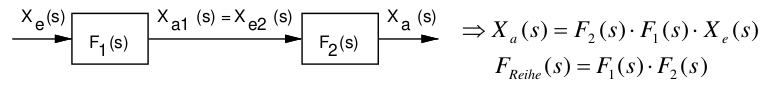
\includegraphics[width=0.9\columnwidth]{Figures/systemtechnik/Kettenstruktur.png}
	      \end{center}

	\item Parallelstruktur:
	      \begin{center}
		      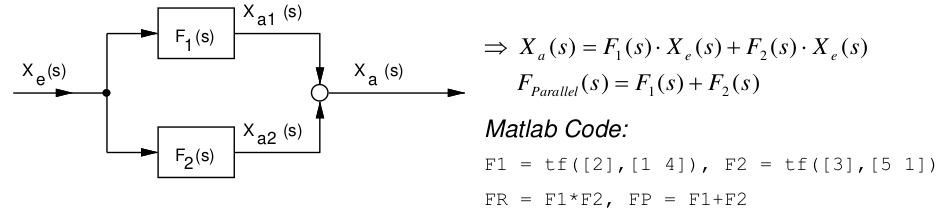
\includegraphics[width=0.9\columnwidth]{Figures/systemtechnik/Parallelstruktur.png}
	      \end{center}

	\item Kreisstruktur:
	      \begin{center}
		      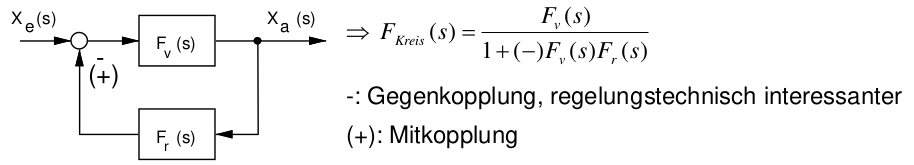
\includegraphics[width=0.9\columnwidth]{Figures/systemtechnik/Kreisstruktur.png}
	      \end{center}

	\item Verschieben einer Additionsstelle:
	      \begin{center}
		      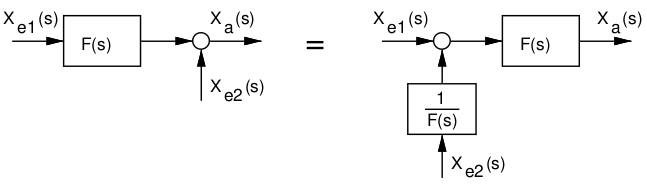
\includegraphics[width=0.9\columnwidth]{Figures/systemtechnik/Verschiebung_Additionsstelle.png}
	      \end{center}

	\item Verschieben einer Verzweigung:
	      \begin{center}
		      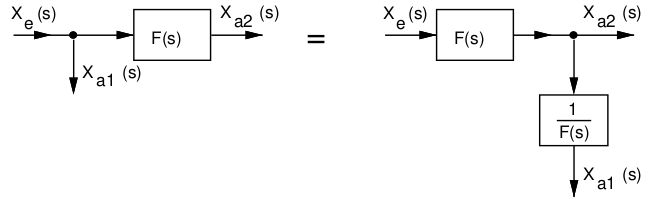
\includegraphics[width=0.9\columnwidth]{Figures/systemtechnik/Verschiebung_Verzweigung.png}
	      \end{center}
\end{itemize}

	\section{Zusammenwirken mehrerer Systeme}
\subsection{Regelkreis}
	\begin{mdframed}[style=exercise, frametitle=Wichtige Begriffe]
		\begin{itemize}[leftmargin=*]
			\item Führungsgröße: w(t)
			\item Störgröße: z(t)
			\item Regelgröße: x(t)
			\item Regeldifferenz: e(t) = w(t) - x(t)
			\item Maximale Überschwingweite: maximale Regelabweichung nach dem erstmaligen Erreichen des Sollwertes
			\item Anregelzeit: Zeit zum erstmaligen Erreichen des Sollwertes
			\item Ausregelzeit: Zeit zum dauerhaften Erreichen des Sollwertes im Toleranzband
		\end{itemize}
	\end{mdframed}

	\begin{mdframed}[style=exercise,frametitle=Anforderungen:]
		\begin{itemize}[leftmargin=*]
			\item Stabilität: Regelkreis muss stabiles Verhalten zeigen (gilt
				auch für instabile Systeme)
			\item Gutes Führungsverhalten: Die Differenz zw. Sollwert w(t) und
				Istwert x(t) muss schnell klein werden.
			\item Gutes Störverhalten: Einfluss von Störgrößen soll vermindert
				werden.
		\end{itemize}
	\end{mdframed}

	Grundstruktur des einschleifigen Regelkreises:

	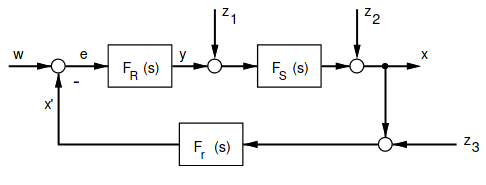
\includegraphics[width=0.8\columnwidth]{Figures/zusammenwirkenMehrererSysteme/einschleifigerRegelkreis.png}

	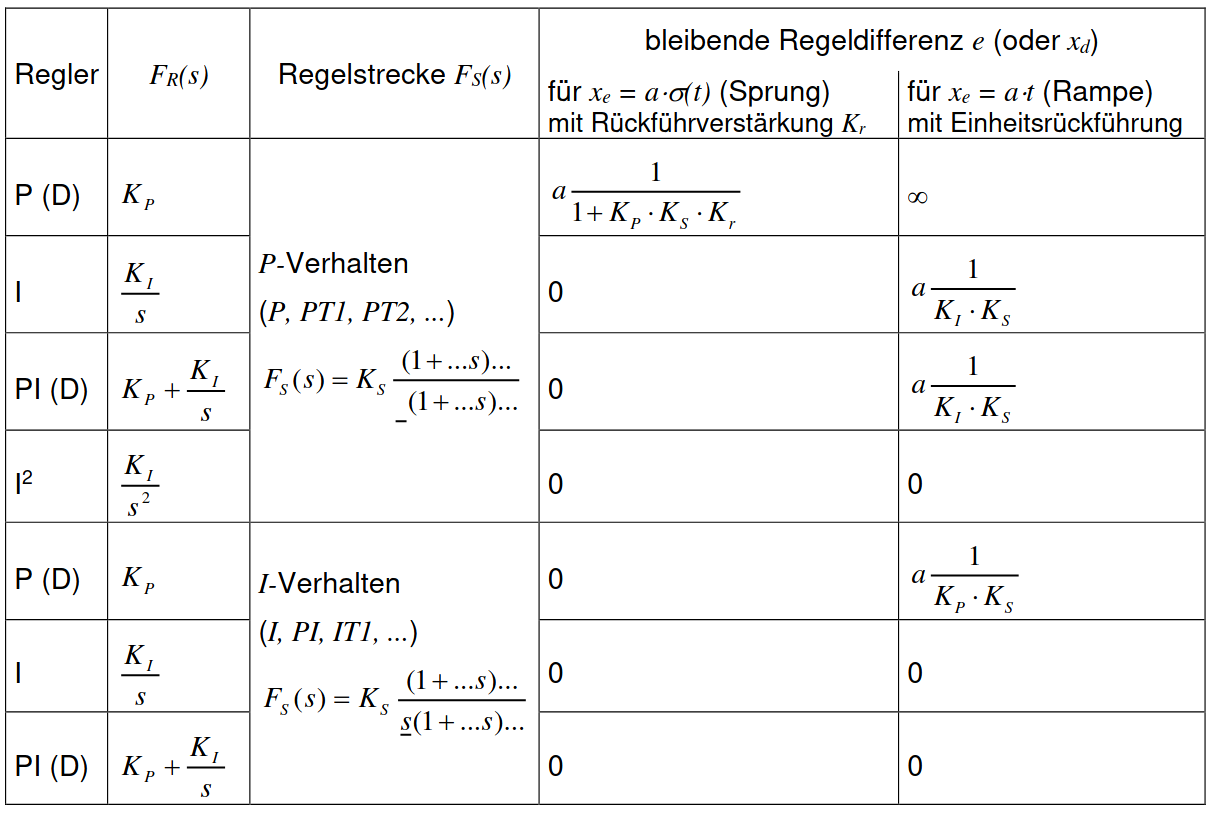
\includegraphics[width=\columnwidth]{Figures/zusammenwirkenMehrererSysteme/Reglerauswahl.png}

	Grundsätzliche Eigenschaften der Kreisstruktur: 

	\begin{figure}[H]
			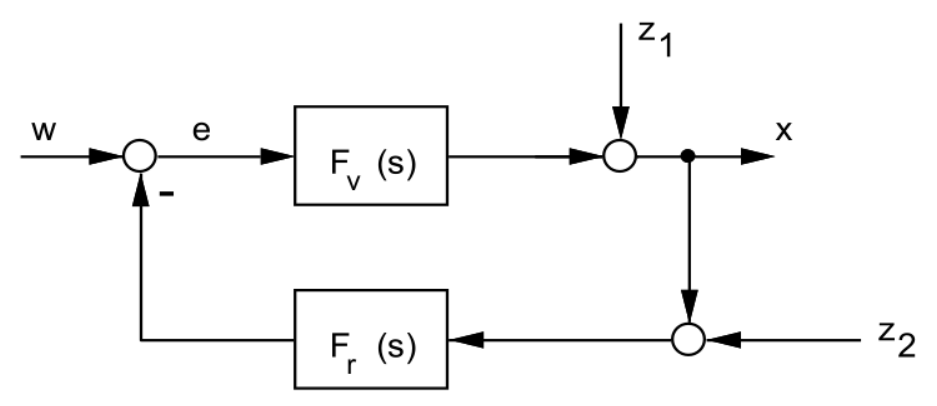
\includegraphics[width=0.8\columnwidth]{Figures/zusammenwirkenMehrererSysteme/Kreisstruktur.png}
	\end{figure}
	\begin{align*}
		X &= \frac{F_V}{1+F_V \cdot F_r}\cdot W + \frac{1}{1 + F_V \cdot F_r} \cdot Z_1 + \frac{- F_V \cdot F_r}{1 + F_V \cdot F_r} \cdot Z_2 \\
		F_w &= \frac{F_V}{1+F_V \cdot F_r} \text{ (Führungsübertragungsfunktion)}\\
		F_{z1} &= \frac{1}{1 + F_V \cdot F_r} \text{ (Störübertragungsfunktion 1)}\\
		F_{z2} &= \frac{- F_V \cdot F_r}{1 + F_V \cdot F_r} \text{ (Störübertragungsfunktion 2)}
	\end{align*}

\subsection{Wurzelortskurven (WOK)-Verfahren}
	\begin{mdframed}[style=exercise]
		Reglerfunktion $F_R$ in Reglerverstärkung und Reglerdynamik aufspalten:
		$F_R =K \cdot F_R ' $
	\end{mdframed}

	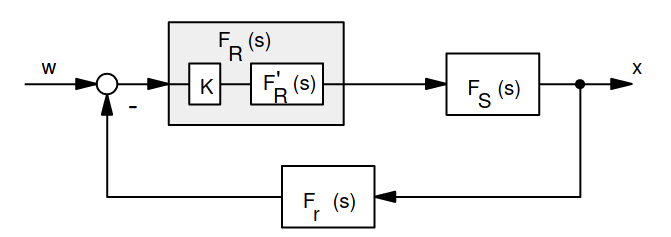
\includegraphics[width=0.94\columnwidth]{Figures/zusammenwirkenMehrererSysteme/WOKkreis.png}\\
	\(
		\Rightarrow F_w (s)= \dfrac {F_R \cdot F_S} {1+F_R \cdot F_S \cdot F_r} = \dfrac {F_R \cdot F_S} {1+F_o}
	\)

	\begin{align*}
		F_o (s) & = F_R (s) \cdot F_S (s) \cdot F_r (s) \\
		& =K \cdot F_R '(s) \cdot F_S (s) \cdot F_r (s) \\
		& =K \cdot Q \cdot \frac{\prod_{\mu=1}^{m}\left(s-s_{\color{red}{N0\mu}}\right)}{\prod_{\vartheta=1}^{n}\left(s-s_{\color{red}{P0\vartheta}}\right)}
	\end{align*}

	Für eine Polstelle muss der Nenner von $F_w (s)$ Null werden:
	\begin{align*}
		\dfrac{F_R (s) \cdot F_S (s)}{1+F_o (s)} \Rightarrow 1+F_o (s) \stackrel{!}{=}0 \\
		\Rightarrow \frac{\prod_{\vartheta=1}^{n}\left(s-s_{\color{red}{P0\vartheta}}\right)}{\prod_{\mu=1}^{m}\left(s-s_{\color{red}{N0\mu}}\right)} = -K \cdot Q
	\end{align*}

	Diese Gleichung kann in Betrag und Phase aufgeteilt werden:
	\begin{align*}
		& \frac{\prod_{\vartheta=1}^{n}\left|s-s_{\color{red}{P0\vartheta}}\right|}{\prod_{\mu=1}^{m}\left|s-s_{\color{red}{N0\mu}}\right|} = |K \cdot Q|
	\end{align*}
	Falls keine Nullstellen vorliegen, ist der Nenner zu 1 zu wählen.
	\begin{align*}
		& \sum_{\vartheta=1}^{n} \angle\left(s-s_{\color{red}{P0\vartheta}}\right) - \sum_{\mu=1}^{m} \angle\left(s-s_{\color{red}{N0\mu}}\right) = \angle\left(-K \cdot Q\right) = \pm r \cdot 180^\circ \\
		& \qquad r = 1,3,5,\ldots \text{ für }K \cdot Q > 0 \\
		& \qquad r = 0,2,4,\ldots \text{ für }K \cdot Q < 0
	\end{align*}

	Aus der Phasenbeziehung lässt sich der Verlauf der WOK bestimmen.\\
	{\footnotesize Wenn Betragsbedingung erfüllt \textrightarrow Punkt ist Teil der WOK}
	\\
	\\
	Die Betragsbeziehung gestattet es, jedem Punkt der WOK den entsprechenden \(K\)-Wert zuzuordnen. \\
	{\footnotesize 
		entsprechenden \(s\)-Wert einsetzen \\
		\(K_{Krit}\) durch einsetzen von \(s_{Krit}\) (Punkt an dem WOK durch Imaginär-Achse geht)\\
		Stabilität für \(K > K_{Krit}\) oder \(K < K_{Krit}\) aus der WOK ablesen.
	}

	\begin{mdframed}[style=exercise, frametitle=Konstruktion der WOK]
		\begin{enumerate}[leftmargin=*]
			\item Alle n Äste der WOK beginnen mit K=0 in den n Polen $s_{Po_v}$ des offenen Regelkreises.
			\item m Äste der WOK enden für K $\rightarrow \pm \infty$ in den \(m\) endlichen Nullstellen $s_{No_v}$ des offenen Regelkreises 
			\item \(n - m\) Äste der WOK enden für K $\rightarrow \pm \infty$ im Unendlichen. \(n - m\) ist der Polüberschuss.
			\item Die n-m ins Unendliche strebende Äste der WOK haben Asymptoten, die\\
				a) im Wurzelschwerpunkt
				\begin{align*}
					s_{w}=\frac{\sum_{v=1}^{n} s_{pov}-\sum_{u=1}^{m} s_{_{Nop}}}{n-m}
				\end{align*}
				beginnen und die dabei\\
				b) mit der reellen Achse die Winkel
				\begin{align*}
					\varphi_{k} &= \frac{(2 k-1) \cdot 180^{\circ}}{n-m} \text{ für } KQ > 0 \\
					\text{bzw. } \varphi_{k} &= \frac{(2 k-2) \cdot 180^{\circ}}{n-m} \text{ für } KQ < 0 \\
					\text{mit } k &= 1,2,3,\ldots,n-m
				\end{align*}
				einschließen.
			\item Die Punkte der WOk liegen entweder auf der reelen Achse, oder symmetrisch zur reelen Achse
			\item Ein Punkt s auf der reellen Achse ist dann ein Punkt der WOK, wenn sich bei KQ > 0 (KQ<0)
				rechts von ihm eine ungerade (gerade) Anzahl von Polen $s_{Po_v}$ und (+) Nullstellen $s_{No_v}$ befindet.
		\end{enumerate}

		Achtung: WOK ist nicht anwendbar, wenn es sich um nicht rationale
		Übertragungsfunktionen handelt.\\ (z.B. Regelkreis mit Totzeitverhalten!)
	\end{mdframed}

\subsection{Nyquist Kriterium}
	\begin{center}
		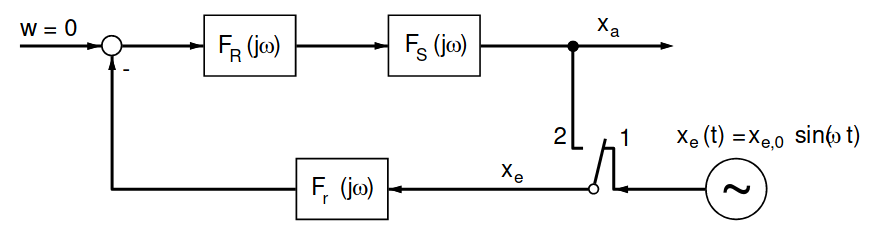
\includegraphics[width=.45\textwidth]{Figures/zusammenwirkenMehrererSysteme/Nyquist.png}
	\end{center}
	Frequenzgangfunktion des offenen Regelkreises:
	\begin{align*}
		F_o (j\omega) = F_r (j\omega) \cdot F_R (j\omega) \cdot F_S (j\omega)
	\end{align*}

	Ausgangssignal:
	\begin{align*}
		x_a(t) &= -F_o (j\omega) \cdot x_e (t)
	\end{align*}

	Regler und seine Parameter werden so gewählt,\\ dass $\omega = \omega_{krit}$ gilt:
	\begin{align*}
		F_o (j\omega_{krit})=-1 \texttt{ (Schwingbedingung)}
	\end{align*}

	\begin{mdframed}[style=exercise]
		Die Schwingbedingung ist erfüllt, wenn die Ortskurve von $F_o (j\omega)$
		durch den kritischen Punkt ($P_{krit} = -1+j0$) der komplexen $F_o$-Ebene
		geht.

		An diesem Punkt kann man $\omega_{krit}$ ablesen (damit kann der Regelkreis
		Dauerschwingungen ausführen).

		Für größere Verstärkung ist das System instabil, für kleinere stabil.
	\end{mdframed}

	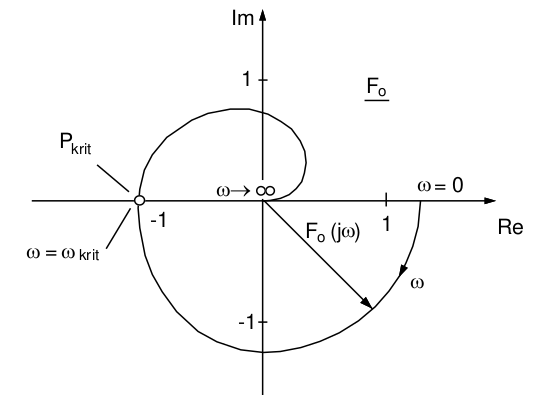
\includegraphics[width=0.94\columnwidth]{Figures/zusammenwirkenMehrererSysteme/Nyquistwkrit.png}

	\begin{mdframed}[style=exercise, frametitle=vereinfachtes Nyquist-Kriterium:]
		Falls F(s) des offenen Kreises keine Pole in der rechten Halbebene hat und
		nur max. 2 im Ursprung der s-Ebene, ist der Regelkreis stabil, wenn: \\
		Beim Durchlaufen der Ortskurve von $F_o (j\omega)$ für $\omega$ von 0 bis $\infty$ der
		kritische Punkt \(F_o(j \omega_{krit} = -1 + 0j)\) auf der linken Seite der Ortskurve liegt.
	\end{mdframed}

	Zur Auswertung des Nyquist-Kriteriums im Bode Diagramm, spaltet man die Ortskurve nach Betrag
	A = $|F_0 (jw)|$ und Phase $\varphi$ = $arg(F_0(jw))$

	\begin{figure}[H]
		\centering
		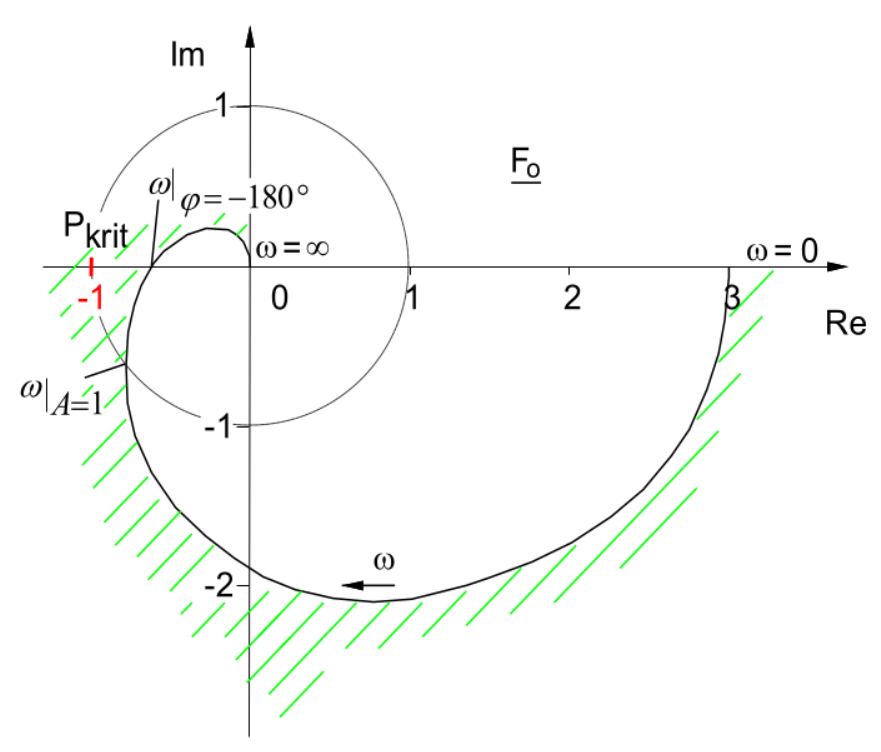
\includegraphics[width=0.6\columnwidth]{Figures/zusammenwirkenMehrererSysteme/Nyquist_Bode_1.png}
		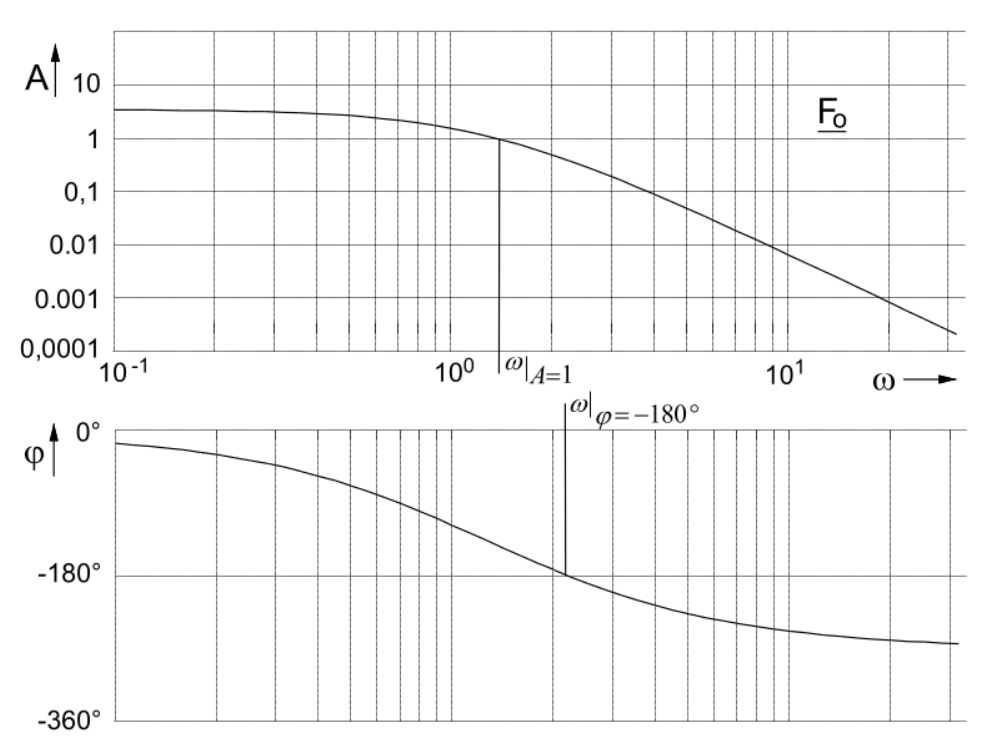
\includegraphics[width=\columnwidth]{Figures/zusammenwirkenMehrererSysteme/Nyquist_Bode_2.png}
	\end{figure}

	\begin{center}
		\textbf{Stabilität für: } \(\left. \omega \right|_{A=1} < \left. \omega \right|_{\varphi = -180^\circ}\)
	\end{center}


	\textbf{Falls die vereinfachte Bedingung nicht funktioniert, wird die allgemeine Formulierung verwendet:}

	\begin{mdframed}[style=exercise, frametitle=Allgemeines Nyquist-Kriterium:]
		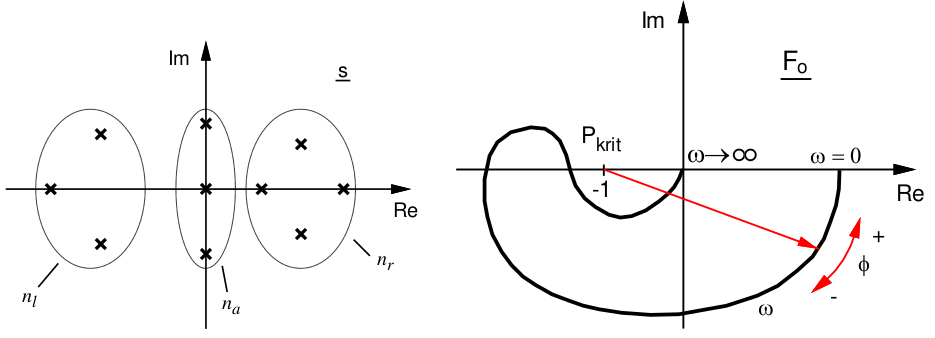
\includegraphics[width=0.94\columnwidth]{Figures/zusammenwirkenMehrererSysteme/Allgemein_Nyquist.png}

		Der geschlossene Regelkreis ist stabil, wenn der Fahrstrahl von $P_{krit}$ = -1 +j0
		zu $F_0 (jw)$ für wachsendes $\omega$ von +0 bis +$\infty$ eine Winkeländerung
		\begin{align*}
			^{\omega=+\infty}_{\omega=+0} \Delta \phi _{soll} = n_r \cdot 180^\circ +n_a \cdot 90^\circ
		\end{align*}
		erfährt.\\
		$n_r$: Anzahl der Pole rechts der imaginären Achse\\
		$n_a$: Anzahl der Pole auf der imaginären Achse
	\end{mdframed}


\begin{minipage}{\columnwidth}
	\subsection{Reglerauslegung im Bode Diagramm}
		Folgende Anforderungen für einen Regler: 
		\begin{mdframed}[style=exercise]
			\begin{itemize}[leftmargin=*]
				\item kleine bleibende Regeldifferenz: \(A(\omega) \gg 1 \text{ bei } \\ \omega \ll \left.\omega\right|_{A=1} \)
				\item Stabilität: \( \left.\varphi\right|_{A=1} > -180^\circ\)
				\item Phasenrand: \(\varphi_R = \left.\varphi\right|_{A=1} + 180^\circ\)\\
					befriedigendes Störverhalten: \(\varphi_R \ge 30^\circ\) \\
					gutes Führungsverhalten (überschwindungsarm): \(\varphi_R \approx 60^\circ\) \\
					gutes Führungsverhalten (überschwingungsfrei): \(\varphi_R \ge 80^\circ\) 
				\item Unterdrückung von Störgrößen: \(A(\omega) \ll 1 \text{ bei } \\ \omega \gg \left.\omega\right|_{A=1} \)
			\end{itemize}
		\end{mdframed}
\end{minipage}

		

\subsection{Einstellregeln}
	\subsubsection{Zeigler/Nichols}
		Zur Bestimmung der Reglerparameter wird der Regelkreis zunächst mit einem reinen P-Regler betrieben. 
		Dabei wird die Reglerverstärkung \(K_P\) so lange erhöht, bis der Regelkreis Dauerschwingungen ausführt.
		Diese kritische Verstärkung \(K_{P,krit}\) und die Periodendauer \(T_{krit}\) der Schwingung werden notiert.
		\begin{figure}[H]
			\centering
			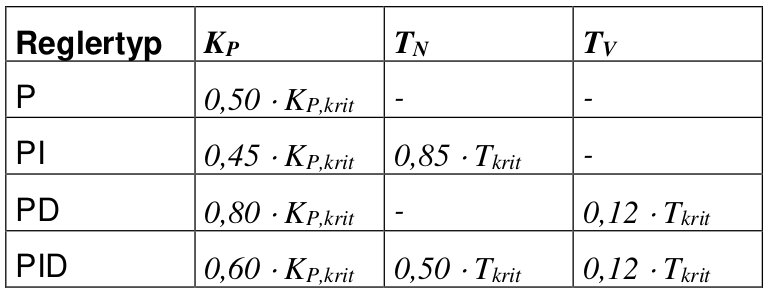
\includegraphics[width=0.9\columnwidth]{Figures/zusammenwirkenMehrererSysteme/ZieglerNich.png}
		\end{figure}		
		Ein Nachteil dieses Verfahrens ist, dass das System bis zum Schwingen gebracht werden muss (Stabilitätsgrenze), was nicht bei allen Regelstrecken zulässig ist (Zerstörung).

	\subsubsection{Betragsoptimum}
		Anwendbar für Systeme mit Streckenverhalten \(PT_n\) mit einer „dominierenden“ (großen) und mehreren kleinen Zeitkonstanten (möglichst reelle Pole):\\
		{ \footnotesize Berechnung inklusive des Rückführteils}
		\begin{align*}
			&T_1 = T_d \gg T_2, T_3, \ldots, T_n \qquad T_\Sigma = \sum T_2, T_3, \ldots, T_n\\
			&\text{Streckenverstärkung: } K_S = K_1 \cdot K_2 \cdot \ldots \cdot K_n \\
			&\Rightarrow \text{PI-Regler: } F_{PI} = K_R \cdot \left(1 + \frac{1}{T_N \cdot s}\right)\\
			&\text{mit } T_N = T_d \quad \text{;} \quad K_R = \frac{T_d}{2 \cdot K_S \cdot T_\Sigma}
		\end{align*}

	\subsubsection{Symmetrisches Optimum}
		Anwendbar für Systeme mit Streckenverhalten \(IT_n\) (reelle Pole notwendig):\\
		{ \footnotesize Berechnung inklusive des Rückführteils}
		\begin{align*}
			&T_\Sigma = \sum T_1, T_2, \ldots, T_n \\
			&\text{Streckenverstärkung: }K_S = K_1 \cdot K_2 \cdot \ldots \cdot K_n \\
			&\Rightarrow \text{PI-Regler} (\varphi_R \approx 40^\circ): \\
			&F_{PI} = K_R \cdot \left(1 + \frac{1}{T_N \cdot s}\right) \\
			&\text{mit } T_N = 4 \cdot T_\Sigma \quad K_R = \frac{1}{2 \cdot K_S \cdot T_\Sigma}
		\end{align*}
		


\subsection{Maßnahmen zur Verbesserung des Regelverhaltens}
	\raggedright
	\begin{mdframed}[style=exercise, frametitle=Störgrößenaufschaltung:]
		Falls Angriffsort einer Störgröße bekannt und Störgröße messbar,kann man wie im Bild kompensieren.\\
		Vorteil: einfacher Regler Entwurf, deutlich schnellere Ausregelung.
	\end{mdframed}
	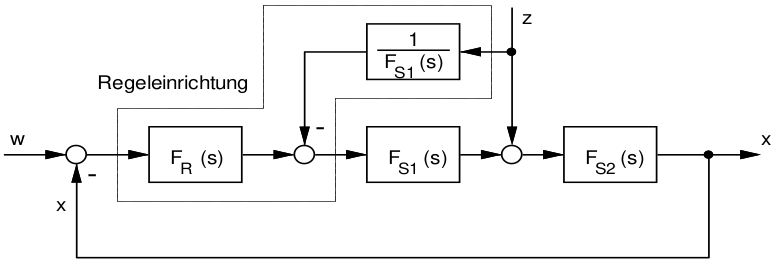
\includegraphics[width=0.9\columnwidth]{Figures/zusammenwirkenMehrererSysteme/Stoergoesenschaltung.png}

	\begin{mdframed}[style=exercise, frametitle=Vorsteuerung:]
		Geeignet, falls kein Kompromiss für gutes Stör und Folgeverhalten.\\
		Regler ist auf gutes Störverhalten ausgelegt. Mit $F_{Rv}$ wird ein schnelles Folgen
		auf Führungssignale w(t) erreicht.
	\end{mdframed}
	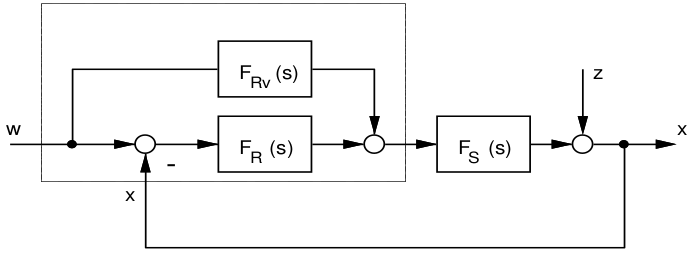
\includegraphics[width=0.9\columnwidth]{Figures/zusammenwirkenMehrererSysteme/Vorsteuerung.png}

	\begin{mdframed}[style=exercise, frametitle=Kaskadenregelung:]
		Ineinander geschachtelte Regelkreise (innere Regelkreise „schneller“). „Innere“
		Störungen können bereits innen ausgeregelt werden. Können von Innen nach Außen in Betrieb genommen werden.

		In WOK: \(K\) für innere Kreise muss festgelegt werden. Dann Integration des „fertigen“ inneren Reglers in größere Reglerstruktur. 
	\end{mdframed}
	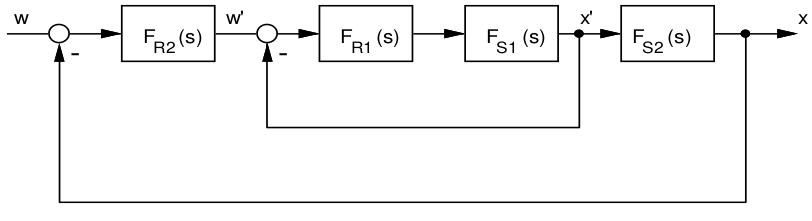
\includegraphics[width=0.9\columnwidth]{Figures/zusammenwirkenMehrererSysteme/Kaskadenregelung.png}

	\begin{mdframed}[style=exercise, frametitle=Führungsgrößenfilter:]
		Falls eine Nullstelle den Regelkreis dominiert (nächster zur Imaginärachse) kommt es zu einem einzelnen Überschwinger. \\
		Zur Vermeidung wird in den Zweig der Führungsgröße ein \(PT_1\)-Filter eingefügt, welches die Nullstelle genau kompensiert.
	\end{mdframed}

	\begin{mdframed}[style=exercise, frametitle=Anti-Windup:]
		Wenn ein Regler mit I-Anteil und eine Begrenzung der Stellgröße vorliegt, kann es zum „Windup“ kommen: I-Anteil wird immer größer, da die Stellgröße begrenzt ist. Dies führt zu Überschwingen. \\
		Anti-Windup: Begrenzung des I-Anteils, damit er nicht über die Stellgrößenbegrenzung hinauswächst.
	\end{mdframed}

	\section{Digitale Regler}

Betrachtung \textbf{quasi-kontinuierlicher Regler}, d.h. \(T_A \le \frac{1}{10} \ldots \frac{1}{20} \cdot T_{System, dom}\) \\
(\(T_{System, dom}\) ist die dominierende (größte) Zeitkonstante des Systems)

\subsection{z-Transformation}

	Wert der bei t = k $\cdot T_A$ ausgegeben wird, wird bei t = (k-1) $\cdot T_A$
	eingelesen. (Verzögerung um einen Abtastschritt):

	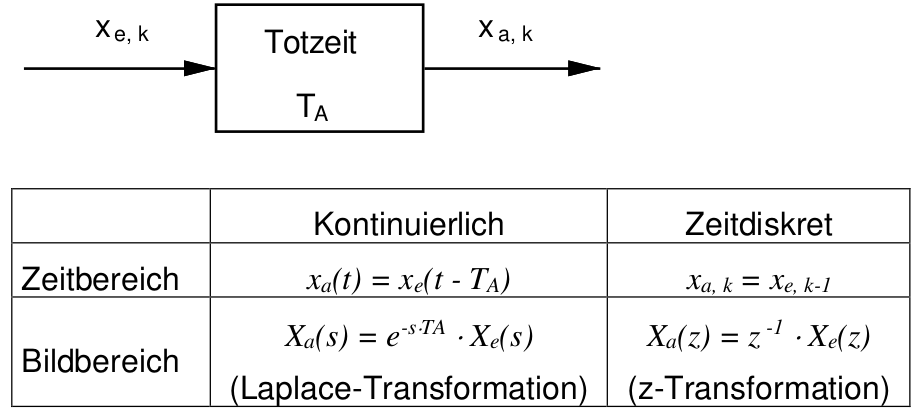
\includegraphics[width=0.9\columnwidth]{Figures/digitaleRegler/zTrans.png}

	\begin{align*}
		\Rightarrow &z \ \hat{=}\  e^{s \cdot T_A} \\
		\text{bzw. } &s \ \hat{=}\  \frac{1}{T_A} \cdot \ln(z)
	\end{align*}

	Um die Übertragungsfunktion eines digitalen Reglers zu erhalten, wird für \(s\) ein entsprechender Ausdruck in Abhängigkeit von \(z\) und der Abtastzeit \(T_A\) eingesetzt. \\ 
	Zur Vereinfachung der Berechnung von digitalen Reglern können folgende Näherungsformeln verwendet werden:

	\begin{itemize}
		\item Rückwärts-Differenzen-Quotient: \(s \ \hat{=} \ \frac{z-1}{T_A \cdot z}\)
		\item Vorwärts-Differenzen-Quotient: \(s \ \hat{=} \ \frac{z-1}{T_A}\)
		\item Tustinsche Formel: \(s \ \hat{=} \ \frac{2}{T_A} \cdot \frac{z-1}{z+1}\)
	\end{itemize}

	\subsubsection{Stabilität von digitalen Reglern}
		Ein digitaler Regler ist stabil, wenn alle Pole innerhalb des Einheitskreises liegen, d.h. \(|z| < 1\). \\
		\textbf{Beispiel:} \(G(z) = \frac{z}{z-0.5}\) hat einen Pol bei \(z = 0.5\) und ist damit stabil, da \(|0.5| < 1\). \\
		\textbf{Beispiel:} \(G(z) = \frac{z}{z-1.5}\) hat einen Pol bei \(z = 1.5\) und ist damit instabil, da \(|1.5| > 1\).

\subsection{Algorithmus aus der Übertragungsfunktion}
	\begin{itemize}
		\item Übertragungsfunktion in z-Form umwandeln
		\item Zähler und Nenner durch die höchste Potenz von z teilen (Es darf nur \(z^0, z^{-1}, z^{-2} \ldots\) geben, kein \(z^{+\ldots}\))
		\item Zähler gibt Eingangsgrößen an, Nenner gibt Ausgangsgrößen an, z.B. \(\frac{2+4z^{-1}}{8-5z^{-1}} \ \Rightarrow \ 8 x_{a,k} - 5 x_{a,k-1} = 2 x_{e,k} + 4 x_{e,k-1} \) 
		\item Umsortierung nach aktueller Ausgangsgröße \(x_{a,k}\) (hier: \(x_{a,k} = \frac{2}{8} x_{e,k} + \frac{4}{8} x_{e,k-1} + \frac{5}{8} x_{a,k-1}\))
	\end{itemize}

	\begin{lstlisting}[language=Matlab]
	while (1) 
	{
		wait_timerinterrupt(TA) //Abtastzeit warten

		xaalt1 = xa
		xealt1 = xe
		input(xe)
		xa = 0.25 * xe + 0.5 * xealt1 + 0.625 * xaalt1
		output(xa)
	}
	\end{lstlisting}
	\section{Systembeschreibung im Zustandsraum}
\subsection{Allgemein (Mehrgrößensystem MIMO) }
	\begin{mdframed}[style=exercise]
		\vspace{-1em}
		\begin{align*}
			\dot{\Vec{x}}(t) & = A\vec{x}(t) + B\vec{u}(t) \quad x(0) = x_{0} \\
			\vec{y}(t)       & = C\vec{x}(t) + D\vec{u}(t)
		\end{align*}
	\end{mdframed}

	\begin{center}
		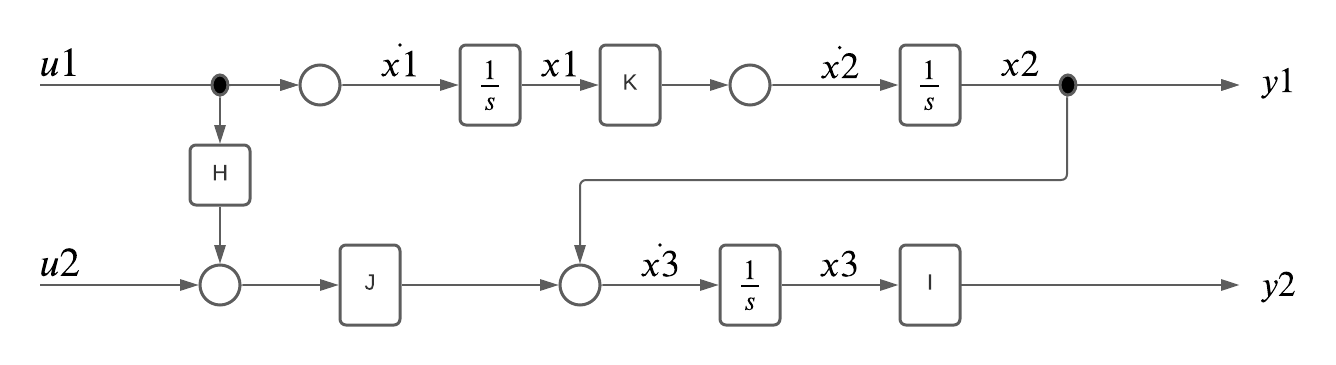
\includegraphics[width=0.96\columnwidth]{Figures/zustandsraum/Signalflussplan.png}
		\captionof{figure}{Signalflussplan}
	\end{center}

	\begin{mdframed}[style=exercise]
		\begin{align*}
			\dot{x}_{1} & = 0\cdot x_{1} +0\cdot x_{2} +0\cdot x_{3} +1\cdot u_{1}+0\cdot u_{2}        \\
			\dot{x}_{2} & = K\cdot x_{1} +0\cdot x_{2} +0\cdot x_{3} +0\cdot u_{1}+0\cdot u_{2}        \\
			\dot{x}_{3} & = 0\cdot x_{1} +0\cdot x_{2} +0\cdot x_{3} +H\cdot J\cdot u_{1}+J\cdot u_{2} \\
			\dot{y}_{1} & = 0\cdot x_{1} +1+x_{2} +0\cdot x_{3} +0\cdot u_{1}+0\cdot u_{2}             \\
			\dot{y}_{2} & = 0\cdot x_{1} +0\cdot x_{2} +l\cdot x_{3} +0\cdot u_{1}+0\cdot u_{2}        \\
		\end{align*}
	\end{mdframed}

	\begin{mdframed}[style=exercise]
		\[A = \begin{bmatrix}
				0 & 0 & 0 \\
				K & 0 & 0 \\
				0 & 0 & 0
			\end{bmatrix} \ 
			B = \begin{bmatrix}
				1         & 0 \\
				0         & 0 \\
				H\cdot{}J & J
			\end{bmatrix}\]
		\[C = \begin{bmatrix}
				0 & 1 & 0 \\
				0 & 0 & l \\
			\end{bmatrix} \
			D = \begin{bmatrix}
				0 & 0 \\
				0 & 0
			\end{bmatrix}
		\]
	\end{mdframed}

	Eigenwerte der A-Matrix liefern Pole:\\
	\begin{align*}
		\operatorname{det}(A - sI) \overset{!}{=} 0
	\end{align*}

\subsubsection{Polfestlegung durch vollständige Zustandsrückführung}

\centering
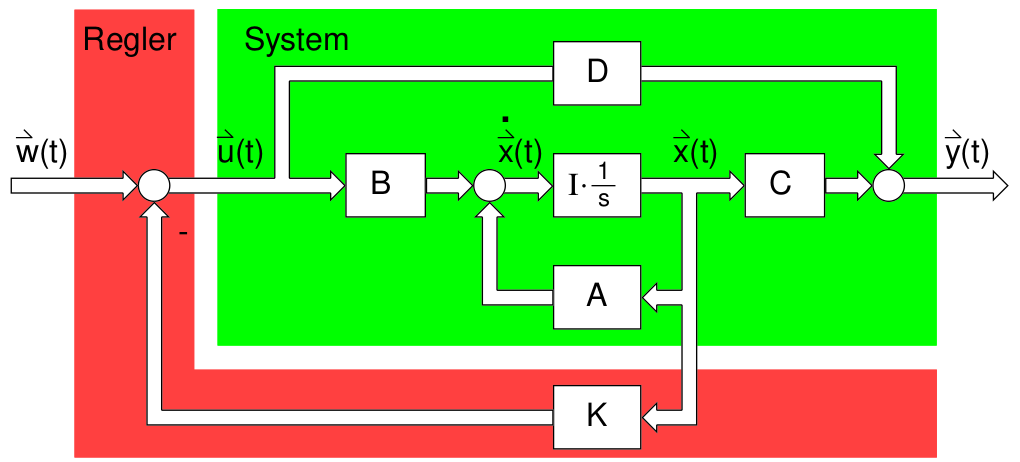
\includegraphics[width=0.8\columnwidth]{Figures/zustandsraum/Polfestlegung.png}

\raggedright
Durch die freie Wahl von K können alle n Pole des Systems beliebig platziert
werden.

Von jeder Zwischengröße \(x_i\) eine Rückführung auf jede Eingangsgröße \(u_j\) mit einem Verstärkungsfaktor \(K_{ij}\) möglich.\\
Die Rückführung führt zu einem neuen System, bei dem die Eingangsgröße \(u_j\) durch die Rückführung von \(x_i\) beeinflusst wird.\\
Zur Bestimmung der neuen Systemmatrix \(A_{RK}\) nach der Rückführung wird die Rückführungsmatrix \(K\) in die ursprüngliche Systemmatrix \(A\) integriert.

Die neue Systemmatrix \(A_{RK}\) muss die gewünschten Pole erhalten.
\begin{align*}
	&\operatorname{det}(A_{RK} - sI) \overset{!}{=} 0 \\
	\Rightarrow &\operatorname{det}(A_{RK} - sI) \overset{!}{=} \text{Nenner von } F(s)_{\text{gew\"unscht}}
\end{align*}


\end{multicols*}
\end{document}
